\chapter{Kiểm tra kiểu - Type checking}
\label{chap:typechecking}
Chương này trình bày cách giải quyết bài toán Kiểm tra kiểu thông qua các bước sau:
\begin{itemize}
\item Mở rộng ngôn ngữ assembly để lưu trữ thông tin về kiểu union.
\item Kiểm tra tính hợp lệ của việc sử dụng kiểu union trong thân chương trình.
\end{itemize}

Các phần tiếp theo của chương sẽ trình bày lần lượt các bước này.

\begin{comment}
\section{Chỉnh sửa để Boomerang chấp nhận việc sử dụng biến không phải thanh ghi}
\subsection{Cơ chế lưu trữ tên thanh ghi hiện nay của Boomerang}
Khi chuyển đổi từ mã assembly sang mã trung gian, Boomerang sẽ dùng một class con của Expr để biểu diễn thanh ghi. Cụ thể là class Location, và gọi phương thức static của class Location là Location::regOf(int num). Ta sẽ truyền vào phương thức này một con số đại diện cho thanh ghi đó. Cặp số - tên thanh ghi này được lưu vào một từ điển, để sau này khi thực hiện phân tích xong thì sẽ chuyển lại từ thanh ghi thành biến cục bộ.

Trong phần giải mã từ mã assembly sang mã trung gian, có một hàm để map giữa tên thanh ghi và con số đại diện cho nó, đó là hàm map\_sfr(string name).
\begin{lstlisting}[caption={Một số phần mã trong hàm map\_sfr},label={list:listmapsfr}]
if (name == "R0") return 0;
else if (name == "R1") return 1;
else if (name == "R2") return 2;
...
else return -1;

\end{lstlisting}

Sau khi trải qua các quá trình phân tích và đến giai đoạn in ra mã đầu ra, trình dịch ngược sẽ gọi hàm getRegName trong class FrontEnd để trả lại tên ban đầu của thanh ghi. Trong hàm getRegName sẽ lấy từ điển tên thanh ghi - số đại diện được quy định sẵn của mỗi phần giải mã cho các kiến trúc máy khác nhau, tìm tên thanh ghi tương ứng với con số đó và trả về.
\begin{lstlisting}[caption={Phần mã trong hàm getRegName},label={list:listgetregname}]
std::map<std::string, int, std::less<std::string> >::iterator it;
for (it = decoder->getRTLDict().RegMap.begin();	 it != decoder->getRTLDict().RegMap.end(); it++)
if ((*it).second == idx) 
return (*it).first.c_str();
return NULL;a
\end{lstlisting}


Như vậy, có thể thấy với các tên biến không được quy định trước, hàm map\_sfr sẽ trả về giá trị -1, và vì giá trị -1 sẽ không có trong từ điển của phần giải mã, nên hàm getRegName sẽ trả về NULL, dẫn đến trình dịch ngược sẽ bị lỗi runtime và dừng ngay lập tức.\\

%lấy mã Boomerang ban đầu về, hiện kết quả khi sử dụng biến đầu vào

Vì số lượng tên biến là rất nhiều, nên ta không thể sử dụng phương pháp thêm mới các tên biến vào từ điển được quy định sẵn được, mà phải có cách để trình dịch ngược linh động hơn, chấp nhận bất kỳ các tên nào được sử dụng trong mã assembly. Giải pháp đưa ra là ngoài việc sử dụng từ điển thanh ghi được quy định sẵn, ta sẽ lập thêm một bảng tên biến, thành phần bao gồm các cặp tên biến - số đại diện. Trong giai đoạn giải mã, khi hàm map\_sfr được gọi, nếu tên truyền vào nằm trong các thanh ghi đã quy định sẵn, thay vì trả về giá trị -1 thì ta sẽ tạo ra một giá trị random và đưa chúng vào bảng tên biến ở trên. Ngoài ra, còn có một đoạn mã kiểm tra biến được sử dụng đã được khai báo bằng câu lệnh \#DEFINE chưa (ngoại trừ một số biến đặc biệt được tự sinh). \\
\begin{lstlisting}[caption={Phần mã mới được bổ sung trong hàm map\_sfr},label={list:listmapsfrnew},language=c++]
bool isDefined = false;
map<char*, AssemblyArgument*>::iterator it;
for (it = replacement.begin(); it!=replacement.end(); it++){
if(strcmp((*it).first, name.c_str()) == 0 ){
isDefined = true;
break;
}
}
if (isDefined || name.find("specbits") != string::npos ){
if (symbolTable->find(name) == symbolTable->end()){
bool existed = false;
int num;
do{
num = std::rand()%200+31;
map<string, int>::iterator it;
for (it = symbolTable->begin(); it!=symbolTable->end(); it++){
bool cond1 = (*it).second == num;
bool cond2 = (byteVar != -1 && byteVar>=num);
bool cond3 = (bit != -1 && bit>=num);
if (cond1 || cond2 || cond3){
existed = true;
continue;
} else {
existed = false;
}
}
} while (existed); 
(*symbolTable)[name] = num;
if (name.find("specbits") != string::npos){
std::cout<<"Name: "<<name<<", "<<num<<endl;
}
return num;
} else {
return symbolTable->find(name)->second;
}
}
else {
std::cout<<"ERROR: "<<name<<" HAS NOT BEEN DEFINED YET"<<endl;
exit(1);
}
\end{lstlisting}
Tương ứng với sự thay đổi ở hàm map\_sfr,  ở hàm getRegName, ngoài việc dò trong từ điển quy định trước, ta sẽ thêm một đoạn mã để dò trong bảng tên biến. 
\begin{lstlisting}[caption={Phần mã mới được bổ sung trong hàm getRegName},label={list:listgetregnamenew},language=c++]
std::map<string,int>::iterator symIt;
for (symIt = decoder->getSymbolTable().begin(); symIt != decoder->getSymbolTable().end(); symIt++){
	if ((*symIt).second == idx){
		return (*symIt).first.c_str();
	}
}
\end{lstlisting}
Như vậy, vấn đề giữ nguyên tên biến được giải quyết mà không ảnh hưởng nhiều tới trình dịch ngược.
%đoạn mã đầu vào assembly và mã đầu ra giữ nguyên được tên biến
\end{comment}
\section{Mở rộng ngôn ngữ assembly}
Để kiểm tra được tính hợp lệ khi sử dụng kiểu union trong đoạn mã đầu vào, trình dịch ngược cần phải được cung cấp thông tin về các kiểu union thông qua một phương thức nào đó. Có hai hướng để giải quyết vấn đề này là:
\begin{itemize}
	\item Đưa ra một cấu trúc khai báo mới cho ngôn ngữ assembly. Cấu trúc khai báo này có thể tương tự như khai báo union ở ngôn ngữ cấp cao. Tuy nhiên, cách làm này sẽ làm cho đoạn mã assembly không thể compile được vì các assembler không chấp nhận cấu trúc mới thêm vào đó.
	\item Cho phép người lập trình đưa các thông tin về kiểu union vào trong phần chú thích theo một mẫu quy định từ trước. Với giải pháp này, đoạn mã không bị ảnh hưởng vì chú thích là một thành phần đã có sẵn trong ngôn ngữ assembly, và khi compile thì các assembler sẽ bỏ qua phần chú thích.
\end{itemize}
Như vậy, giải pháp thứ hai là tối ưu hơn và sẽ được áp dụng trong luận văn này. Mẫu chú thích được viết cho 8051 được thể hiện ở đoạn mã \ref{list:listdeclarevar}
\begin{lstlisting}[caption={Mẫu khai báo bộ biến},label={list:listdeclarevar}]
;BEGIN DEFINE
;DEFINE BYTE
[byte var declare]
;DEFINE BITS
[eight bit var declares]
;END DEFINE
\end{lstlisting}
Tuy nhiên, cũng giống như assembler, các trình dịch ngược hầu như sẽ bỏ qua phần chú thích khi đọc đoạn mã đầu vào, và để cho trình dịch ngược có thể rút trích được thông tin từ phần chú thích thì phải thực hiện một số chỉnh sửa trong giai đoạn lexer và parser, cụ thể là:
\begin{itemize}
	\item Chỉnh sửa lexer để nhận biết các token là những chú thích đặc biệt. Như trong ví dụ \ref{list:listdeclarevar}, các chú thích \textbf{";BEGIN DEFINE"}, \textbf{";DEFINE BYTE"}, \textbf{";DEFINE BITS"} không thể được đọc vào như là token \textit{COMMENT} bình thường, mà phải có những token riêng biệt cho chúng để phục vụ giai đoạn parser. Đoạn mã \ref{list:8051lexer} được viết để chạy trên thư viện \textit{flex++} thể hiện điều đó. Có thể thấy, khi bắt được một chú thích, thay vì trả về token \textit{COMMENT} như trước đó, phần lexer mới này sẽ kiểm tra nội dung chú thích, nếu trùng với các chú thích đặc biệt thì sẽ trả về token tương ứng. 
\end{itemize}
\begin{changemargin}{0cm}{0cm} 
	\begin{lstlisting}[caption={Phần lexer được chỉnh sửa để nhận biết các chú thích đặc biệt},label={list:8051lexer}]
	(\;.*)  { 
		string beginDefine = ";BEGIN DEFINE";
		string endDefine = ";END DEFINE";
		string defineByte = ";DEFINE BYTE";
		string defineBits = ";DEFINE BITS";
		string val = strdup(yytext);
		if (beginDefine == val)
			return BEGINDEFINE;
		else if (endDefine == val)
			return ENDDEFINE;
		else if (defineByte == val)
			return DEFINEBYTE;
		else if (defineBits == val)
			return DEFINEBITS;
		else return COMMENT;
		}
	\end{lstlisting}

\end{changemargin} 
\begin{itemize}
	\item Chỉnh sửa parser để nhận vào cấu trúc khai báo union. Tiếp tục với ví dụ mẫu khai báo \ref{list:listdeclarevar}, nếu phần parser chỉ đọc các câu lệnh khai báo biến bình thường, thì không thể xác định được các union mà người dùng khai báo trước. Như vậy, cần chỉnh sửa parser để bắt được những mẫu khai báo đặc biệt. Phần parser viết bằng thư viện \textit{bison++} cho mẫu khai báo \ref{list:listdeclarevar} được trình bày ở đoạn mã \ref{list:8051parser}. Trước khi chỉnh sửa, phần parser này chỉ có luật \textit{define}, đọc vào từng câu lệnh khai báo độc lập. Sau khi được chỉnh sửa lại, luật \textit{definebit} có độ ưu tiên cao hơn sẽ đọc vào cấu trúc khai báo union gồm nhiều câu lệnh khai báo khác nhau.
\end{itemize}
\begin{changemargin}{0cm}{0cm} 
	\begin{lstlisting}[caption={Đoạn mã parser nhận biết các mẫu khai báo union},label={list:8051parser}]
	definebit: BEGINDEFINE END_LINE DEFINEBYTE END_LINE 
					define DEFINEBITS END_LINE defineeachbit{8} 
					ENDDEFINE END_LINE;
	defineeachbit: DEFINE ID bit END_LINE;
	define:	DEFINE ID expressions END_LINE;
	\end{lstlisting}
\end{changemargin} 
\begin{itemize}
	\item Chỉnh sửa các hành động sau khi parser nhận biết được những cấu trúc khai báo union. Sau khi parser đã bắt được các mẫu khai báo union, cần lập trình để lưu trữ thông tin về các union đó vào dữ liệu của chương trình. Cấu trúc được dùng để lưu trữ thông tin về union này là \textit{UnionDefine}, được trình bày ở đoạn mã \ref{list:listuniondefine}, trong đó, \textit{byteVar} để lưu trữ tên của union đó, còn \textit{bitVar} chứa các thành phần thuộc union và vị trí vùng nhớ mà thành phần đó truy xuất. Đoạn mã \ref{list:8051parser2} thể hiện phần code đưa các khai báo union từ mã đầu vào thành các thực thể \textit{UnionDefine} tương ứng.
\end{itemize}
\begin{changemargin}{0cm}{0cm} 
	\begin{lstlisting}[caption={Cấu trúc dữ liệu để lưu trữ một union},label={list:listuniondefine},language=c++]
	class UnionDefine{
		public:
			char* byteVar;
			map<int, char*>* bitVar;
	};
	\end{lstlisting}
	\begin{lstlisting}[caption={Đoạn mã parser bao gồm các hành động sau khi nhận biết được union},label={list:8051parser2}]
	definebit: BEGINDEFINE END_LINE DEFINEBYTE END_LINE 
					define DEFINEBITS END_LINE defineeachbit{8} 
					ENDDEFINE END_LINE
	{
		UnionDefine* ut = new UnionDefine();
		$5 -> expList -> pop_back();
		ut->byteVar = $5 -> expList -> back() -> 
		argList.back()->value.c;
		ut->bitVar = bitVar;
		unionDefine1 -> push_back(ut);
		bitVar = new map<char*, int>();
	};
	defineeachbit: DEFINE ID bit END_LINE {
		std::string temp($3->value.c);
		char c =  temp.at(temp.size()-1);
		int num = c - '0';
		(*bitVar)[$2] = num;
	};
	define: DEFINE ID expressions END_LINE 
	{ 
		AssemblyLine* line = new AssemblyLine();
		line -> expList = new list<AssemblyExpression*>();
		line->kind = INSTRUCTION;
		line->name = "DEFINE";
		AssemblyExpression* expr1 = new AssemblyExpression();
		expr1 -> kind = UNARY;
		Arg a;
		a.c=$2;
		expr1 -> argList.push_back(new AssemblyArgument(6, a));
		line -> expList->push_back(expr1);
		line->expList ->push_back(expr);//*/
		expr = new AssemblyExpression();
		$$=line;
	};
	\end{lstlisting}
\end{changemargin} 
	
Như vậy, sau khi thực hiện các chỉnh sửa trên, trình dịch ngược đã có thể đọc vào các thông tin về union được người dùng cung cấp ở phần chú thích của đoạn mã đầu vào, đồng thời lưu trữ thông tin đó vào cấu trúc dữ liệu \textit{UnionDefine}. Tuy đã xác định được những union nào được khai báo trong mã đầu vào, nhưng cần phải có một bước để kiểm tra những union đó có được sử dụng hợp lý hay không.
\section{Kiểm tra tính hợp lệ của việc sử dụng kiểu union}
Như đã trình bày ở phần \ref{sec:challenge}, ngôn ngữ assembly không cho phép thao tác trực tiếp trên các vùng nhớ, mà phải thông qua một thanh ghi trung gian và việc sử dụng một thành phần \textit{y} thuộc union \textit{x} chỉ hợp lệ khi mà thanh ghi trung gian đang mang kiểu union \textit{x} đó. Thông thường, mỗi kiến trúc máy sẽ có một thanh ghi trung gian đặc trưng, ví dụ như với 8051 là thanh ghi \textit{ACC}. Như vậy, quá trình kiểm tra kiểu union sẽ gồm 2 bước:
\begin{itemize}
	\item Xác định kiểu của thanh ghi trung gian tại mỗi điểm của chương trình.
	\item Kiểm tra việc truy xuất thành phần của union có hợp lý hay không.
\end{itemize}
\subsection{Xác định kiểu của thanh ghi trung gian}
Trong quá trình nghiên cứu, có 2 giải pháp được đưa ra để xác định kiểu của thanh ghi:
\begin{itemize}
	\item Sử dụng phương pháp phân tích Reaching definitions (đã được giới thiệu ở phần \ref{sec:reachdef}), lập trình thêm phần mở rộng để xác định thông tin về kiểu từ tập câu lệnh gán tìm được.
	\item Sử dụng phương pháp Lan truyền kiểu - Type propagation để lan truyền kiểu của thanh ghi theo luồng đi của chương trình.
\end{itemize}
Hai giải pháp này được trình bày lần lượt ở các phần tiếp theo.
\subsubsection{Phân tích Reaching definitions kết hợp phần mở rộng}
Phân tích Reaching definitions cho biết được tại một thời điểm của chương trình, các câu lệnh gán nào đang còn có giá trị, nhưng thông tin đó là chưa đủ để biết được kiểu dữ liệu của thanh ghi trung gian. Nếu câu lệnh tìm thấy được là một câu lệnh gán trực tiếp vùng nhớ có địa chỉ là một biến khai báo trước cho thanh ghi, thì dễ dàng xác định được kiểu của thanh ghi là union mang tên biến đó. Tuy nhiên, thực tế cho thấy biểu thức quy định địa chỉ vùng nhớ cho thanh ghi có nhiều dạng khác nhau, cụ thể là:
\begin{itemize}
		\item Một hằng số.
	\item Một thanh ghi, giá trị của thanh ghi có thể được khai báo ở các câu lệnh trước đó.
	\item Một biểu thức có hai vế, các vế của biểu thức có thể là một biến, một thanh ghi hoặc một hằng số.
\end{itemize}
Ví dụ về các câu lệnh gán vùng nhớ cho thanh ghi viết bằng mã 8051 được thể hiện ở đoạn mã \ref{list:listhardcase}. Phương pháp Reaching definitions sẽ không thể xử lý được khi gặp các câu lệnh gán này. Ở câu lệnh số 1, phân tích có thể lấy được giá trị \textbf{38H}, nhưng không thể xác định được biến nào đã được khai báo giá trị \textbf{38H}. Ở câu lệnh số 2, Reaching definitions không thể biết được giá trị của thanh ghi \textit{DPTR} là bao nhiêu. Ở câu lệnh số 3, việc xử lý lại càng phức tạp hơn, vì nếu chỉ đơn giản lấy biểu thức vế phải \textit{OPTIONS+1} của khai báo ra, không thể nào biết được giá trị thực sự của nó là bao nhiêu. \\
\begin{lstlisting}[caption={Một số câu lệnh gán trên 8051 mà Reaching definitions không xử lý được},label={list:listhardcase}]
MOV A, 38H ;1
MOV A, @DPTR ;2
MOV A, OPTIONS+1 ;3
\end{lstlisting}
Ngoài ra, trong đoạn mã \ref{list:ifcond}, tại thời điểm câu lệnh sử dụng biến bit \textit{TESTSUPS}, có hai câu lệnh khai báo biến \textit{a}. Đối với phương pháp Reaching definitions, nó sẽ xem như có hai giá trị mà biến \textit{a} có thể mang. Tuy nhiên, nếu xét kỹ hơn, thì sẽ thấy là cả hai giá trị đó đều là biến \textit{OPTIONS}, và thực chất tại thời điểm này \textit{a} chỉ mang một giá trị, cho dù luồng đi của chương trình có như thế nào. Như vậy, phương pháp Reaching definitions sẽ bỏ qua những trường hợp như thế này và dẫn đến việc độ chính xác sẽ không được cao.
\begin{lstlisting}[caption={Đoạn mã có nhiều câu lệnh khai báo cho ACC đến được một điểm của chương trình nhưng tất cả đều cùng giá trị},label={list:ifcond}]
if (...){
	a = *(OPTIONS);
	...
} else {
	a = *(OPTIONS);
	...
}
TESTSUPS = 1;
\end{lstlisting}
Để khắc phục những khuyết điểm trên của phương pháp Reaching definitions, cần có một phần mở rộng để xử lý được những trường hợp gán phức tạp. Ý tưởng cho phần mở rộng đó như sau:
\begin{itemize}
	\item Đối với địa chỉ vùng nhớ là hằng số: Vì trong quá trình parser, trình dịch ngược có lưu trữ thông tin về tên biến và giá trị của biến đó vào một danh sách dữ liệu, nên có thể tìm kiếm trong danh sách đó ra được tên biến và đó cũng là tên của union mà thanh ghi đang mang.
	\item Đối với địa chỉ vùng nhớ là một thanh ghi khác: Kiểm tra tập các câu lệnh gán còn giá trị tại thời điểm đó của chương trình, sẽ tìm ra được biểu thức giá trị của thanh ghi đó. Áp dụng giải thuật của phần mở rộng lên biểu thức đó để tìm ra giá trị thực sự của thanh ghi và trả về. Nếu giá trị trả về là một biến được khai báo trước, thì tên biến là kiểu union cần tìm.
	\item Đối với địa chỉ vùng nhớ là một biểu thức hai toán hạng: Hiện tại, phần mở rộng không thể xử lý được trường hợp này, do việc tính toán giá trị của một biểu thức hai toán hạng là khá phức tạp. Đây là một trong những khuyết điểm của phần mở rộng.
\end{itemize}
Cụ thể các bước giải thuật của phần mở rộng được trình bày ở hình \ref{fig:reachdefextendalgo}.
\begin{figure}
	\centering
	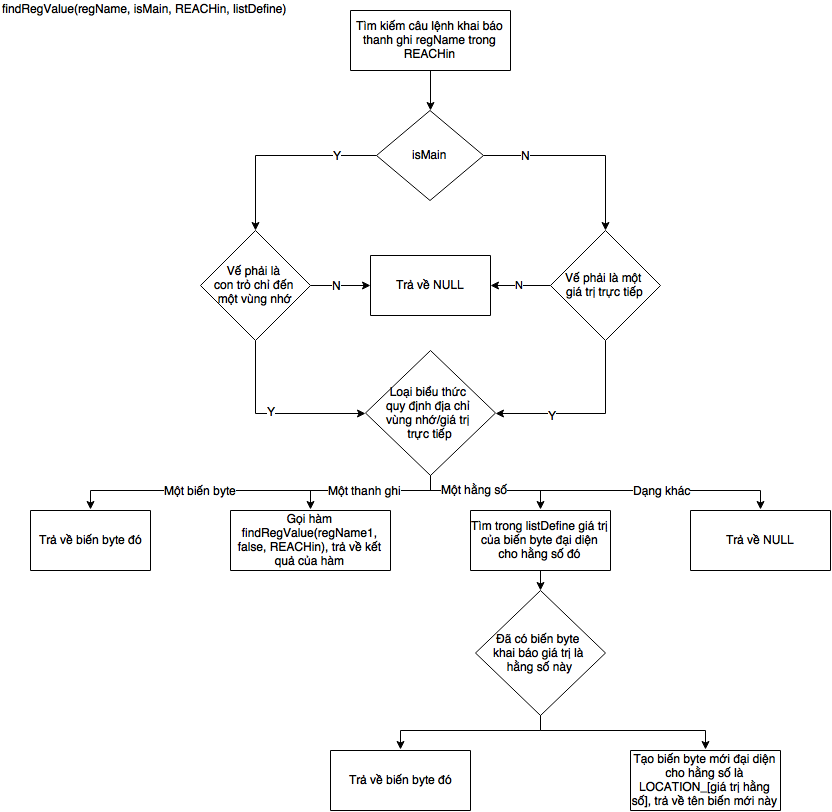
\includegraphics[width=\linewidth]{image/reachdefextendalgo}
	\caption{Giải thuật cho hàm findRegValue - phần mở rộng của phân tích Reaching definitions}
	\label{fig:reachdefextendalgo}
\end{figure}

Theo giải thuật nêu trên, cần truyền vào cho hàm \textit{findRegValue} các giá trị sau đây:
\begin{itemize}
	\item \textit{regName}: Tên thanh ghi cần tìm kiểu dữ liệu
	\item \textit{isMain}: Biến bool cho biết đây có phải là thanh ghi cần xác định kiểu không hay chỉ là thanh ghi trung gian của quá trình xác định kiểu đó. Nếu là thanh ghi cần xác định kiểu, thì biểu thức được xét đến là địa chỉ của vùng nhớ được gán cho thanh ghi, còn nếu không phải, thì biểu thức được xét đến là giá trị trực tiếp của thanh ghi.
	\item \textit{REACHin}: Tập các câu lệnh gán có giá trị đến thời điểm đó của chương trình. Tập này được xây dựng nhờ vào giải thuật Reaching definitions.
	\item \textit{listDefine}: Đây là danh sách lưu trữ các biến được khai báo ở đầu chương trình. Danh sách này gồm các cặp tên biến - giá trị biến.
\end{itemize}

Như vậy, sau khi trải qua phần mở rộng này, nếu thanh ghi trung gian đang mang một kiểu union được khai báo trước thì hàm \textit{findRegValue} sẽ trả về \textbf{tên của kiểu union} đó. Còn nếu không phải thì giá trị trả về là \textbf{NULL}. Đến đây, việc xác định kiểu union của thanh ghi trung gian đã giải quyết xong.\\

Tuy đã xử lý được hầu hết các trường hợp của phép gán vùng nhớ cho thanh ghi, nhưng việc có thêm một phần mở rộng này sẽ làm cho tốc độ xử lý trình dịch ngược giảm đi. Cộng thêm việc bản thân giải thuật Reaching definitions đã có độ phức tạp cao, tổng thời gian xử lý cho bước này của trình dịch ngược là khá lớn. Vì vậy, nhu cầu đặt ra là có một phương pháp khác có độ chính xác tương đương Reaching definitions cộng phần mở rộng, nhưng có thời gian xử lý thấp hơn. Phương pháp này sẽ được trình bày tiếp theo đây.

\subsubsection{Phân tích Lan truyền kiểu - Type propagation}
Phương pháp phân tích Lan truyền kiểu - Type propagation có thể xem là một đóng góp mới của luận văn tốt nghiệp này. Phương pháp này được đặt ra nhằm giải quyết hạn chế về mặt thời gian xử lý của Reaching definitions kết hợp phần mở rộng. Có hai nguyên nhân chính làm thời gian xử lý của phương pháp trên bị chậm là:
\begin{itemize}
	\item Sau khi đã chạy vòng lặp quét các câu lệnh của chương trình, vẫn chưa thể kết luận được kiểu dữ liệu mà thanh ghi đang mang. Phải trải qua một giai đoạn xử lý dữ liệu nữa thì mới rút trích ra được thông tin đó.
	\item Với cách chạy vòng lặp cổ điển thường thấy của các phương pháp phân tích dữ liệu, nếu ở một câu lệnh nào đó có sự thay đổi về tập \textit{REACHin} và \textit{REACHout}, thì toàn bộ các câu lệnh khác trong chương trình đều phải tính toán lại 2 tập trên dù chúng có bị ảnh hưởng hay không.
\end{itemize}
Như vậy, để tăng nhanh thời gian xử lý, phương pháp Lan truyền kiểu có ý tưởng như sau:
\begin{itemize}
	\item Xem thông tin về kiểu union của thanh ghi là một dữ liệu để lan truyền qua các câu lệnh của chương trình. Như vậy, kết thúc quá trình chạy vòng lặp, đã có thể xác định được thanh ghi trung gian đang mang kiểu union gì mà không cần phải xử lý thêm.
	\item Thay vì sử dụng phương pháp chạy vòng lặp, bất cứ câu lệnh nào có thay đổi gì thì sẽ tính toán lại toàn bộ chương trình, thì phương pháp sử dụng worklist sẽ được thay thế. Với phương pháp này, chỉ các câu lệnh có trong worklist mới được tính toán, và khi có thay đổi ở một câu lệnh nào đó, thì chỉ những câu lệnh bị ảnh hưởng bởi sự thay đổi này mới được đưa vào worklist và tính toán.
	\item Sử dụng mã SSA nhằm giúp cho việc tính toán thuận tiện hơn. Chi tiết về công dụng của mã SSA sẽ được phân tích rõ hơn sau khi thuật toán chi tiết được trình bày. Trong các trình dịch ngược, luôn có một giai đoạn mã đầu vào được thể hiện ở dạng SSA để phục vụ cho các quá trình phân tích dữ liệu, nên sẽ không mất thời gian chuyển đổi từ mã thường sang mã SSA.
\end{itemize}
Các ý tưởng trên được thể hiện cụ thể qua giải thuật ở hình \ref{fig:typepropagationalgo}.\\
\begin{figure}[h!]
	\centering
	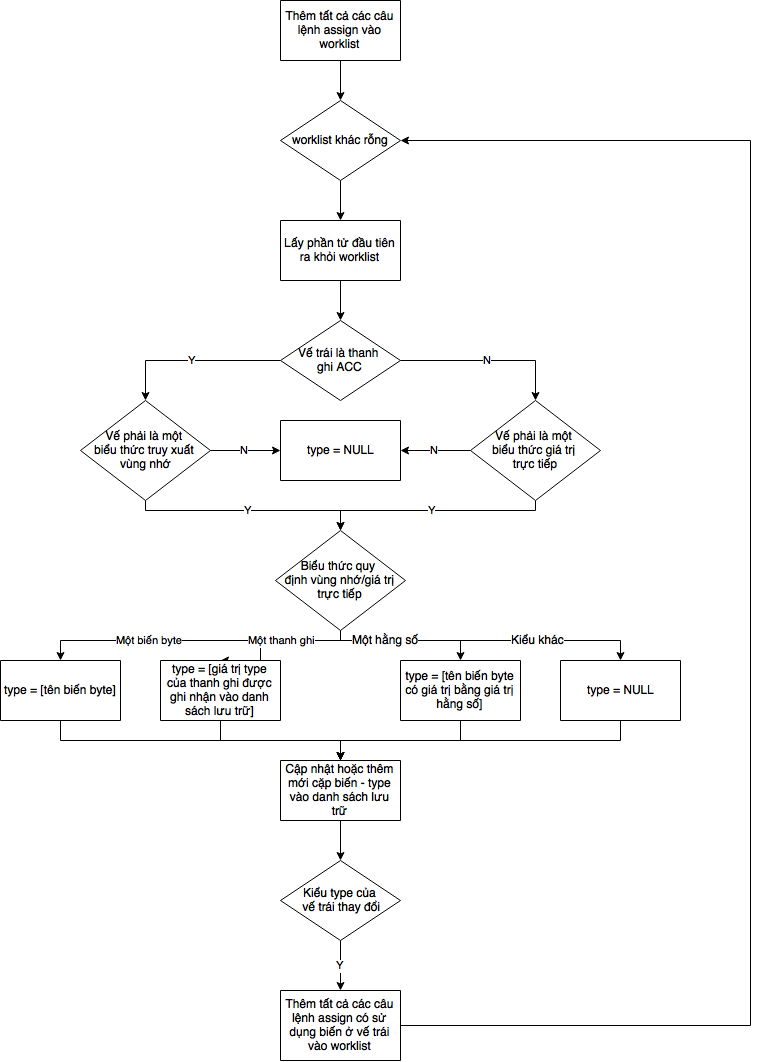
\includegraphics[width=\linewidth]{image/typePropagationAlgo}
	\caption{Giải thuật của phân tích Type propagation}
	\label{fig:typepropagationalgo}
\end{figure}
Từ giải thuật trên, có thể thấy mã SSA mang đến những lợi ích sau:
\begin{itemize}
	\item Tiết kiệm không gian lưu trữ. Vì mỗi biến SSA chỉ được định nghĩa một lần duy nhất, nên chỉ cần một bảng lưu trữ tên biến - kiểu union cho toàn bộ chương trình, không cần thiết ở mỗi câu lệnh phải lưu một tập vào và một tập ra như phương pháp Reaching definitions.
	\item Giúp cho việc tìm các câu lệnh bị ảnh hưởng bởi sự thay đổi của một câu lệnh nào đó dễ dàng hơn. Ở bước cuối của vòng lặp, phải tìm các câu lệnh có sử dụng biến ở vế trái của câu lệnh thay đổi. Nếu đoạn mã đang ở dạng thông thường, thì việc xác định tập câu lệnh này rất khó khăn, do một biến có thể được định nghĩa lại nhiều lần nên phải kiểm tra câu lệnh nào đang sử dụng biến được định nghĩa tại câu lệnh được ghi nhận thay đổi. Nhưng với mã SSA, mỗi biến chỉ được gán một lần duy nhất trong toàn bộ chương trình, nên việc tìm kiếm sẽ dễ dàng hơn rất nhiều.
\end{itemize}

Như vậy, phương pháp Lan truyền kiểu này sẽ làm giảm đáng kể thời gian xử lý của chương trình so với phương pháp Reaching definitions. Tuy nhiên, khuyết điểm của Lan truyền kiểu là vẫn chưa xử lý được trường hợp biểu thức vế phải có hai toán hạng. Để giải quyết được vấn đề này, cần có một phân tích khác mạnh hơn và phân tích đó sẽ được giới thiệu ở chương tiếp theo.
\subsection{Kiểm tra việc truy xuất thành phần của union có hợp lý hay không}

\label{sec:laststep}
Sau khi đã xác định được kiểu của thanh ghi trung gian ở từng thời điểm của chương trình, bước tiếp theo sẽ là kiểm tra tại thời điểm truy xuất thành phần của một union, thanh ghi trung gian có đang mang đúng kiểu union đó không. Việc kiểm tra này là khá đơn giản do đã có thông tin:
\begin{itemize}
	\item Kiểu union và các thành phần của nó từ phần khai báo
	\item Kiểu union của thanh ghi trung gian thông qua quá trình phân tích
\end{itemize}
Như vậy, chỉ cần dò tìm và so trùng hai dữ liệu trên để đưa ra kết quả cuối cùng. Các bước kiểm tra này trình bày ở hình \ref{fig:checkunionsteps}.
\begin{figure}
	\centering
	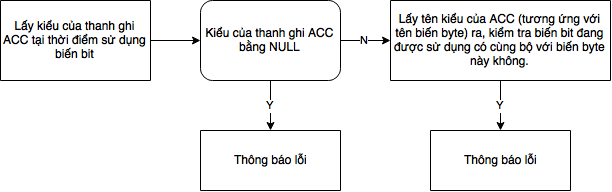
\includegraphics[width=\linewidth]{image/checkUnionSteps}
	\caption{Quá trình kiểm tra một câu lệnh sử dụng bit}
	\label{fig:checkunionsteps}
\end{figure}
Một ví dụ về việc truy xuất thành phần union không hợp lý được thể hiện ở đoạn mã \ref{list:invalid8051}. Trong đoạn mã này, phần khai báo cho thấy \textit{TESTSUPS} là một thành phần thuộc union \textit{OPTIONS}, tuy nhiên ở câu lệnh số 2, khi thực hiện truy xuất thành phần \textit{TESTSUPS}, thanh ghi trung gian là \textit{ACC} lại mang một kiểu union khác là \textit{OPTIONS2}. Như vậy, việc truy xuất này là không hợp lý và phải được cảnh báo để người dùng sửa chữa lại đoạn mã chương trình.
	\begin{lstlisting}[caption={Đoạn mã 8051 chứa một truy xuất thành phần union không hợp lý},label={list:invalid8051}]
;BEGIN DEFINE
;DEFINE BYTE
#DEFINE OPTIONS #38
;DEFINE BITS
#DEFINE TESTSUPS ACC.1
...
;END DEFINE
...
MOV A, OPTIONS2 ;1
SETB TESTSUPS ;2
\end{lstlisting}

Như vậy, với bài toán Kiểm tra kiểu, thông tin về kiểu union đã có sẵn ngay từ đầu và chỉ cần kiểm tra xem người lập trình có thực hiện việc truy xuất các thành phần của union hợp lý không trước khi sinh ra mã ở ngôn ngữ cấp cao. Giải pháp cho bài toán yêu cầu can thiệp vào trình dịch ngược ít và hiện thực dễ dàng. Tuy nhiên, giải pháp còn nhiều hạn chế như phương pháp phân tích dữ liệu chưa đạt độ chính xác cao, cần người dùng phải chỉnh sửa lại chú thích theo mẫu quy định...



